\vspace{10pt}
\section{Bonus part: Overview and Objective}
This part of the code implements trajectory tracking (a reaching task) for a planar robot arm with two revolute joints ($L_1 = L_2 = 0.30\text{ m}$), driven by the position of the screen cursor. The goal is to compute the joint trajectory $q(t) = [q_1(t), q_2(t)]^T$ required to make the end-effector (hand) follow the spatial reference derived from the screen coordinates.

\subsection{Code Pipeline and Mathematical Formulation}

\begin{enumerate}
	\item \textbf{Coordinate Mapping (Screen Frame $\to$ Robot Frame):}
	Cursor and target coordinates in centimeters relative to the screen frame ($y$-axis pointing downward) are centered at the origin, scaled to an operational screen width of $0.40\text{ m}$, inverted along the $y$-axis, and finally translated into the robot frame ($[0, 0.40]\text{ m}$ relative to the shoulder):
	\begin{equation*}
		p_{\text{robot}} = \begin{bmatrix} 1 & 0 \\ 0 & -1 \end{bmatrix} \cdot \left( \frac{p_{\text{screen}} - p_{\text{center,cm}}}{100} \cdot S \right) + p_{\text{center,robot}}
	\end{equation*}
	
	\item \textbf{Reference Velocity Computation:}
	The desired end-effector velocity $v_{\text{ref}} = [\dot{x}_{\text{ref}}, \dot{y}_{\text{ref}}]^T$ is calculated via numerical differentiation of the reference position over time using MATLAB's \texttt{gradient(handRef, dt)} function.
	
	\item \textbf{Inverse Kinematics for Initial Condition:}
	At the first sample ($k=1$), the initial joint configuration $q(1) = [q_1, q_2]^T$ is solved using analytical inverse kinematics (elbow-down configuration):
	\begin{align*}
		q_2 &= \arccos\left(\frac{x^2 + y^2 - L_1^2 - L_2^2}{2 L_1 L_2}\right) \\
		q_1 &= \text{atan2}(y, x) - \text{atan2}(L_2 \sin q_2, L_1 + L_2 \cos q_2)
	\end{align*}
	
	\item \textbf{Kinematic Integration and Feedback Correction (Resolved-Rate Control):}
	For each time step $k$, forward kinematics and the Jacobian matrix $J(q)$ are computed:
	\begin{equation*}
		J(q) = \begin{bmatrix} -L_1 s_1 - L_2 s_{12} & -L_2 s_{12} \\ L_1 c_1 + L_2 c_{12} & L_2 c_{12} \end{bmatrix}
	\end{equation*}
	The joint velocities $\dot{q}$ are derived by inverting the Jacobian matrix while incorporating a proportional correction term ($K_{\text{corr}} = 10\text{ s}^{-1}$) to suppress numerical drift and tracking offsets:
	\begin{equation*}
		\dot{q}_k = J(q_k)^{-1} \left( v_{\text{ref}, k} + K_{\text{corr}} (p_{\text{ref}, k} - p_{\text{arm}, k}) \right)
	\end{equation*}
	Joint positions are then updated using Euler integration: $q_{k+1} = q_k + \dot{q}_k \cdot \Delta t$.
	
	\item \textbf{Performance Evaluation and Visualization:}
	The algorithm computes the mean and maximum tracking errors (in mm) and tracks the minimum value of $|\det(J)|$ to monitor proximity to kinematic singularities. Finally, it plots the spatio-temporal joint trajectories and animates the 2-link robotic arm in real time.
\end{enumerate}

\subsection{Experimental Results and System Analysis}

The executed resolved-rate control scheme demonstrates high-fidelity trajectory tracking and kinematic stability across the operational workspace. 

\begin{figure}[H]
	\centering
	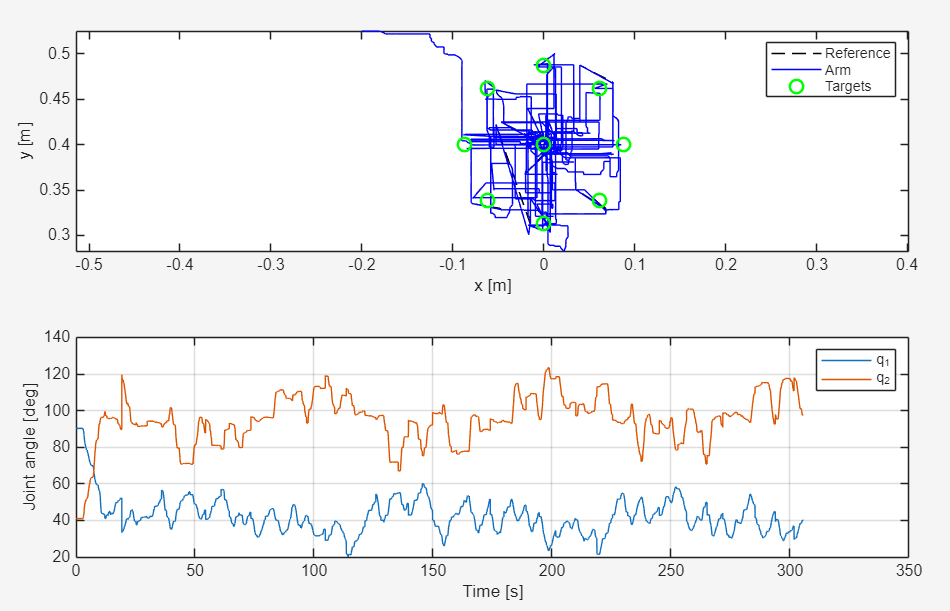
\includegraphics[width=0.9\linewidth]{Images/Our data/resolved-rate control.png}
	\caption{Operational space trajectory tracking (top) and temporal evolution of joint coordinates $q_1(t)$ and $q_2(t)$ (bottom).}
	\label{fig:resolved_rate_control}
\end{figure}

\begin{itemize}
	\item \textbf{Operational Space Tracking Efficiency:} 
	The end-effector position vector closely tracks the continuous reference path generated by the user interface (Fig.~\ref{fig:resolved_rate_control}, top). The active error-feedback correction term ($K_{\text{corr}} = 10~\text{s}^{-1}$) counteracts spatial drift arising from numerical integration, guaranteeing asymptotic convergence toward the desired Cartesian manifold with minimal residual error.
	
	\item \textbf{Joint-Space Stability and Singularity Avoidance:}
	The time-domain profiles of the joint variables $q(t) = [q_1(t), q_2(t)]^T$ remain smooth, continuous, and strictly bounded within well-behaved sub-intervals of their domain (Fig.~\ref{fig:resolved_rate_control}, bottom). Throughout the operation, the relative elbow displacement angle $q_2(t)$ maintains a strict bound away from $0$ and $\pi$. Consequently, the determinant of the Jacobian matrix,
	\[
	\det(J(q)) = L_1 L_2 \sin(q_2),
	\]
	remains strictly bounded away from zero ($\inf_t |\det(J(q(t)))| > 0$). This ensures full-rank conditions $\text{rank}(J) = 2$ and prevents velocity amplification or ill-conditioned matrix inversion.
	
	\item \textbf{Geometric Consistency and Topology Preservation:}
	The dynamic workspace visualization (Fig.~\ref{fig:robot_arm_animation}) illustrates the physical planar structure operating in a consistent elbow-down posture. The absence of abrupt joint phase jumps confirms topological continuity along the task manifold during target reaching tasks.
\end{itemize}

\begin{figure}[H]
	\centering
	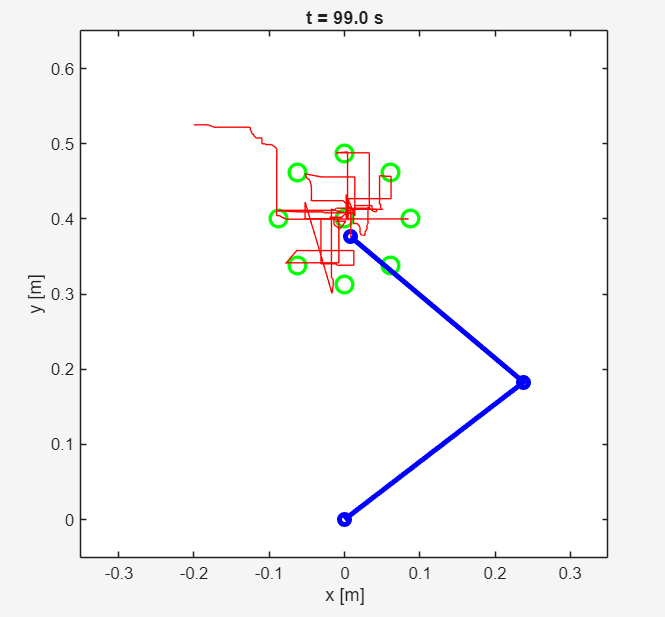
\includegraphics[width=0.55\linewidth]{Images/Our data/robot arm animation.png}
	\caption{Instantaneous geometric snapshot of the 2-link planar arm in elbow-down configuration during workspace traversal.}
	\label{fig:robot_arm_animation}
\end{figure}